\documentclass[landscape,final,a0paper]{baposter}


\tracingstats=2


\usepackage{calc}
\usepackage{graphicx}
\usepackage{amsmath}
\usepackage{amssymb}
\usepackage{relsize}
\usepackage{multirow}
\usepackage{bm}
\usepackage{graphicx}
\usepackage{multicol}

\usepackage{pgfbaselayers}
\pgfdeclarelayer{background}
\pgfdeclarelayer{foreground}
\pgfsetlayers{background,main,foreground}

\usepackage{times}
\usepackage{helvet}
\usepackage{palatino}

\newcommand{\captionfont}{\footnotesize}

\selectcolormodel{cmyk}

%%%%%%%%%%%%%%%%%%%%%%%%%%%%%%%%%%%%%%%%%%%%%%%%%%%%%%%%%%%%%%%%%%%%%%%%%%%%%%%%
% Multicol Settings
%%%%%%%%%%%%%%%%%%%%%%%%%%%%%%%%%%%%%%%%%%%%%%%%%%%%%%%%%%%%%%%%%%%%%%%%%%%%%%%%
\setlength{\columnsep}{0.5em}
\setlength{\columnseprule}{0mm}


%%%%%%%%%%%%%%%%%%%%%%%%%%%%%%%%%%%%%%%%%%%%%%%%%%%%%%%%%%%%%%%%%%%%%%%%%%%%%%%%
% Save space in lists. Use this after the opening of the list
%%%%%%%%%%%%%%%%%%%%%%%%%%%%%%%%%%%%%%%%%%%%%%%%%%%%%%%%%%%%%%%%%%%%%%%%%%%%%%%%
\newcommand{\compresslist}{%
\setlength{\itemsep}{1pt}%
\setlength{\parsep}{0pt}%
\setlength{\parskip}{0pt}%
}

\newcommand{\matlab}{{\scshape Matlab}}
\usepackage[]{mcode}
\usepackage{url}





%%%%%%%%%%%%%%%%%%%%%%%%%%%%%%%%%%%%%%%%%%%%%%%%%%%%%%%%%%%%%%%%%%%%%%%%%%%%%%
%%% Begin of Document
%%%%%%%%%%%%%%%%%%%%%%%%%%%%%%%%%%%%%%%%%%%%%%%%%%%%%%%%%%%%%%%%%%%%%%%%%%%%%%

\begin{document}

%%%%%%%%%%%%%%%%%%%%%%%%%%%%%%%%%%%%%%%%%%%%%%%%%%%%%%%%%%%%%%%%%%%%%%%%%%%%%%
%%% Here starts the poster
%%%---------------------------------------------------------------------------
%%% Format it to your taste with the options
%%%%%%%%%%%%%%%%%%%%%%%%%%%%%%%%%%%%%%%%%%%%%%%%%%%%%%%%%%%%%%%%%%%%%%%%%%%%%%
% Define some colors
\definecolor{silver}{cmyk}{0,0,0,0.3}
\definecolor{yellow}{cmyk}{0,0,0.9,0.0}
\definecolor{reddishyellow}{cmyk}{0,0.4,0.9,0.0}
\definecolor{black}{cmyk}{0,0,0.0,1.0}
\definecolor{darkyellow}{cmyk}{0,0,1.0,0.5}
\definecolor{darkSilver}{cmyk}{0,0,0,0.1}
\definecolor{lighteryellow}{cmyk}{0,0,0.3,0.0}
\definecolor{lightestyellow}{cmyk}{0,0,0.05,0.0}
\definecolor{cyan}{cmyk}{1,0,0,0}
\definecolor{lightcyan}{cmyk}{0.5,0,0,0}
\definecolor{pastelcyan}{cmyk}{0.25,0,0,0}
\definecolor{magenta}{cmyk}{0,1,0,0}
\definecolor{yellow}{cmyk}{0,0,1,0}
\definecolor{lightyellow}{cmyk}{0,0,0.5,0}
\definecolor{pastelyellow}{cmyk}{0,0,0.25,0}
\definecolor{black}{cmyk}{0,0,0,1}
\definecolor{darkgray}{cmyk}{0,0,0,0.75}
\definecolor{gray}{cmyk}{0,0,0,0.5}
\definecolor{lightgray}{cmyk}{0,0,0,0.25}
\definecolor{white}{cmyk}{0,0,0,0}
\definecolor{red}{cmyk}{0,1,1,0}
\definecolor{orange}{cmyk}{0,0.5,1,0}
\definecolor{scarlet}{cmyk}{0,1,0.5,0}
\definecolor{brown}{cmyk}{0.5,0.75,1,0}
\definecolor{camel}{cmyk}{0.25,0.375,0.5,0}
\definecolor{cream}{cmyk}{0,0.2,0.3,0}
\definecolor{green}{cmyk}{1,0,1,0}
\definecolor{lightgreen}{cmyk}{0.5,0,0.5,0}
\definecolor{pastelgreen}{cmyk}{0.25,0,0.25,0}
\definecolor{mossgreen}{cmyk}{0.64,0.4,1,0}
\definecolor{yellowgreen}{cmyk}{0.5,0,1,0}
\definecolor{skyblue}{cmyk}{0.4,0.16,0,0}
\definecolor{royal}{cmyk}{1.0,0.5,0,0}
\definecolor{navyblue}{cmyk}{0.9,0.75,0.5,0}
\definecolor{lightnavy}{cmyk}{0.4,0.3,0.2,0}
\definecolor{blue}{cmyk}{1,1,0,0}
\definecolor{lightblue}{cmyk}{0.5,0.5,0,0}
\definecolor{pastelblue}{cmyk}{0.25,0.25,0,0}
\definecolor{lightpastelblue}{cmyk}{0.15,0.15,0,0}
\definecolor{lightestpastelblue}{cmyk}{0.05,0.05,0,0}
\definecolor{lavender}{cmyk}{0.25,0.25,0,0}
\definecolor{violet}{cmyk}{0.75,1,0.25,0}
\definecolor{purple}{cmyk}{0.5,1,0.5,0}
\definecolor{lightpurple}{cmyk}{0.25,0.5,0.25,0}
\definecolor{pink}{cmyk}{0,0.5,0,0}


%%

\typeout{Poster Starts}
%\background{
  %\begin{tikzpicture}[remember picture,overlay]%
  %  \draw (current page.north west)+(-2em,-2em) node[anchor=north west] %{\hspace{-2em}\includegraphics[height=1.1\textheight]{silhouettes_background}};
 % \end{tikzpicture}%
%}




\begin{poster}%
  % Poster Options, such as colours etc
  {
  columns=4,
  % Show grid to help with alignment
  grid=false,
 % Column spacing
  colspacing=0.5em,
 % Color style
  borderColor=orange,
  headerColorOne=yellow,
  headerColorTwo=lighteryellow,
  headerFontColor=black,
% Format of textbox
  headerborder=open,
  textborder=roundedright,
% Format of text header
  eyecatcher=true,
  headerheight=0.1\textheight,
  headershape=roundedleft,
  headershade=shadetb,
  boxshade=plain,
  background=shadetb,
  bgColorOne=reddishyellow,
  bgColorTwo=lighteryellow,
  boxColorOne=white,
  boxColorTwo=white,
  linewidth=2pt
  }
  % Eye Catcher
  {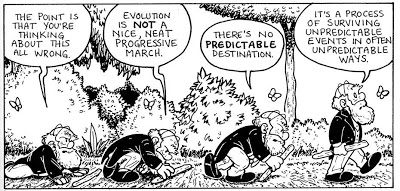
\includegraphics[width=15em]{Darwin-Hosler.png}} 
  % Title
  {\rm
  Darwinian selection in a Boolean network}
  % Authors
  {\rm
    \vspace{1em} 
	Florian Song \hspace{1cm} June 2014
  }
  % University logo
  { % The makebox allows the title to flow into the logo
    \makebox[8em][r]{%
       \begin{minipage}{16em}
				\hfill 
\includegraphics[height=3em]{imperial.pdf}
		\end{minipage}
    }
  }

  \tikzstyle{light shaded}=[top color=baposterBGtwo!30!white,bottom color=baposterBGone!30!white,shading=axis,shading angle=30]

\headerbox{Introduction}{name=intro,column=0,row=0}{
In this poster I will discuss a way to model natural selection as suggested by Charles Darwin.\\ This model uses a Boolean network with the agents/nodes playing local zero-sum games against each other. The outcomes of these games are determined by the \emph{phenotype/strategy} and the \emph{environment} of the agents. The Darwinian update is then performed by replacing the worst performing agent by a new agent with new properties and the above procedure is subsequently repeated.
}
 
 
\headerbox{Motivation}{name=motivation, column=1}{
The model is motivated by natural selection in the sense that certain phenotypes are tested for their fitness in the given environment, formed by other agents. The loser being removed from the system can be thought of as an individual or even a species being submerged by others, because of their unsuccessful strategy. Likewise, the new agent can resemble a mutation within a species which is then on trial for viability being born into the niche of the previously unfit. 
}


\headerbox{Model}{name=model, column=0, span=2, below=intro}{

This project including the model is largely based on and inspired by the article [1], but small alterations were made as appropriate to render the model more coherent and more natural for implementation.\\ As mentioned above, the model revolves around a Boolean network composed of $N$ nodes that can attain the two states $S_i = 0$ or $S_i = 1$ for agent $i$. There are two types of updates, that the network has to undergo:
\begin{enumerate} 
\item {\large The games} (subdivided into two steps):
\begin{enumerate}

\item A series of $N$ games, where each of the agents acts as an {\em aggressor} and is assigned to a random {\em other} agent called the {\em opponent}. In this model, no two agents are mutual aggressors. The games go as follows: \underline{If} $S_{agg} = S_{opp}$ \underline{then} the aggressor scores $+1$ and the opponent $-1$, \underline{otherwise} the aggressor scores $-1$ and the opponent score $+1$.

\item One evolution of the network. For this, every agent is also assigned to $K$ {\em other source} agents. For the remainder of the project, $K = 2$. Now each agent is also associated with a certain Boolean function, that determines the next state of this particular agent. Let the state of agent $i$ at time step $t$ be $S_i(t)$, then
$$ S_i(t) = f_i(S_{i_1}(t-1), S_{i_2}(t-1))$$ 
where $f_i$ is a Boolean function and $S_{i_1}$ and $S_{i_2}$ are the two source agents. This Boolean function is weighted with a parameter $P=\frac{3}{4}$, i.e. three of the four possible inputs $(\{0,0\},\{0,1\},\{1,0\},\{1,1\})$ give the same output whereas the last one gives the other output. This gives $8$ possible $f_i$.\\
{\scshape Note:} This Boolean function is equivalent to the {\em genotype}. Also, the source agents and the opponents constitute the {\em environment}. Together, they eventuate in the agents {\em phenotypic behaviour}.

\end{enumerate}

For the update, step (a) is carried out first, where all $N$ agents participate on average in two games. Then step (b) is parallelly executed for every agent.\\
This is now done repeatedly until an {\em attractor} is found. Since the state space is finite, there is always going to be a certain constellation at a certain time step that occured before. Because the update is entirely deterministic, the sequence inbetween will be repeated to infinity. This is the {\em attractor}. The time to reach it is called the {\em transient}.

\item {\large The Darwinian update} 

In this update, the worst performing agent is the agent with the most negative overall score after the games in step (a). This node is then replaced by a new agent, who is associated with a new Boolean function, new source agents and a new oppenent. These are all chosen at random whilst being careful not to create any mutual aggressors.\\ {\scshape Note:} The connections of other agents involving the loser are not altered. 

\end{enumerate}
}


\headerbox{Implementation}{name=implementation, column=2, row=0, span = 2}{

I implemented this model in \matlab, which might not be the most efficient software package for such a model, but it did a good job overall.\\ 
Many of the ideas how to set this up came from the \matlab \: RBN Toolbox written by Christian Schwarzer. However, this toolbox was not powerful enough for the model, so that a significant amount was altered or added by me. In particular, an effort was made to vectorise most of the existing functions, since large parts of the toolbox were running on \mcode{for} loops. Also, the implementation of the games and the Darwinian update was entirely written by me. 
}



\headerbox{Main Ideas}{name=ideas, column=2, below=implementation}
{
\begin{enumerate}
\item In order to set up the network, a {\em structure array} called ``node'' with quite a few fields was used. Some selected fields are: 


\begin{description}
\item[node.state] The current state i.e. $0$ or $1$
\item[node.nextState] The next state
\item[node.input] Indices of the {\em source agents}
\item[node.rule] A $4\times1$ matrix containing binary entries according to which the next state is determined.
\item[node.score] The score after $N$ games in one time step
\item[node.opp] The index of the opponent
\end{description}

\item A $N\times N$ matrix called ``conn'' specified the connections between the nodes, i.e. the source agents.

\item A $4\times N$ matrix called ``rule'' specified for each node, what the next state is depending on the states of the source agents.
\end{enumerate}
}




\headerbox{Sample Code}{name=code, column=2, below=ideas}{
This is some code showing how I implemented the games. However, it is only a very small part of the code.
\lstinputlisting{Games.m}
}



\headerbox{Results}{name=results, column=3, below=implementation}{
The results presented here are without exception drawn from my own calculations. Because my computing power was rather limited and \matlab \: is known for its weakness with \mcode{for} loops, I was unfortunately not able to get simulations of similar volume. However, by shrinking the size of the network (ie. small $N$), I was able to achieve numbers of iterations close to the ones in the article.\\
Whilst the reference article handled a few different aspects of the model, I focused on the number of updates survived by agents at the time when they are replaced in the Darwinian update. This number is called the {\em lifetime}. Below is a plot produced with my implementation for $N=8$ and $10^5$ iterations of the model:

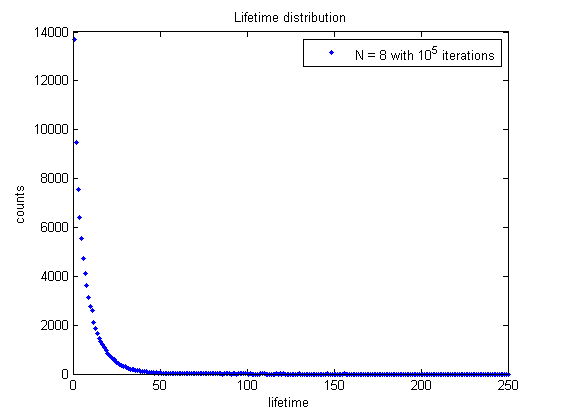
\includegraphics[width=20em]{figure1}

The main result is here, that this suggests power-law-like behaviour where $counts(l) \sim l^{-0.91}$, where $l$ is the lifetime.








}


	
%%%%%%%%%%%%%%%%%%%%%%%%%%%%%%%%%%%%%%%%%%%%%%%%%%%%%%%%%%%%%%%%%%%%%%%%%%%%%%
  \headerbox{References}{name=references,column=3,below=results}{
    \smaller
    \vspace{-0.4em}
    \bibliographystyle{plain}
    \renewcommand{\section}[2]{\vskip 0.05em}
      \begin{thebibliography}{1}\itemsep=-0.01em
      \setlength{\baselineskip}{0.4em}
      \bibitem{article}
        {\bfseries Daniel Eriksson and Henrik Jeldtoft Jensen}
        \newblock {\em Darwinian Selection in a locally unstable Boolean network}
        \newblock published in the Journal of Statistical Mechanics, 2004.
      \bibitem{toolbox}
        {\bfseries Christian Schwarzer (supervised by Christof Teuscher)}
        \newblock {\em \matlab \: RBN Toolbox}
        \newblock Available at: \url{http://www.teuscher.ch/rbntoolbox/}
      \bibitem{eyecatcher}
      {\bfseries Eyecatcher} from \url{satisfactorycomics.blogspot.com}  
      \end{thebibliography}
  \vspace{0.15ex}
  
  }
%%%%%%%%%%%%%%%%%%%%%%%%%%%%%%%%%%%%%%%%%%%%%%%%%%%%%%%%%%%%%%%%%%%%%%%%%%%%%%
  
\end{poster}

\end{document}
